% arara: xelatex
\documentclass[12pt]{article}

% \usepackage{physics}


\usepackage{hyperref}
\hypersetup{
    colorlinks=true,
    linkcolor=blue,
    filecolor=magenta,      
    urlcolor=cyan,
    pdftitle={Overleaf Example},
    pdfpagemode=FullScreen,
    }

\usepackage{tikzducks}

\usepackage{tikz} % картинки в tikz
\usepackage{microtype} % свешивание пунктуации

\usepackage{array} % для столбцов фиксированной ширины

\usepackage{indentfirst} % отступ в первом параграфе

\usepackage{sectsty} % для центрирования названий частей
\allsectionsfont{\centering}

\usepackage{amsmath, amsfonts, amssymb} % куча стандартных математических плюшек

\usepackage{comment}

\usepackage[top=2cm, left=1.2cm, right=1.2cm, bottom=2cm]{geometry} % размер текста на странице

\usepackage{lastpage} % чтобы узнать номер последней страницы

\usepackage{enumitem} % дополнительные плюшки для списков
%  например \begin{enumerate}[resume] позволяет продолжить нумерацию в новом списке
\usepackage{caption}

\usepackage{url} % to use \url{link to web}


\newcommand{\smallduck}{\begin{tikzpicture}[scale=0.3]
    \duck[
        cape=black,
        hat=black,
        mask=black
    ]
    \end{tikzpicture}}

\usepackage{fancyhdr} % весёлые колонтитулы
\pagestyle{fancy}
\lhead{Теория вероятностей и статистика: кнад}
\chead{}
\rhead{Контрольная 2}
\lfoot{}
\cfoot{Да пребудет с тобой сила!}
\rfoot{}

\renewcommand{\headrulewidth}{0.4pt}
\renewcommand{\footrulewidth}{0.4pt}

\usepackage{tcolorbox} % рамочки!

\usepackage{todonotes} % для вставки в документ заметок о том, что осталось сделать
% \todo{Здесь надо коэффициенты исправить}
% \missingfigure{Здесь будет Последний день Помпеи}
% \listoftodos - печатает все поставленные \todo'шки


% более красивые таблицы
\usepackage{booktabs}
% заповеди из докупентации:
% 1. Не используйте вертикальные линни
% 2. Не используйте двойные линии
% 3. Единицы измерения - в шапку таблицы
% 4. Не сокращайте .1 вместо 0.1
% 5. Повторяющееся значение повторяйте, а не говорите "то же"


\setcounter{MaxMatrixCols}{20}
% by crazy default pmatrix supports only 10 cols :)


\usepackage{fontspec}
\usepackage{libertine}
\usepackage{polyglossia}

\setmainlanguage{russian}
\setotherlanguages{english}

% download "Linux Libertine" fonts:
% http://www.linuxlibertine.org/index.php?id=91&L=1
% \setmainfont{Linux Libertine O} % or Helvetica, Arial, Cambria
% why do we need \newfontfamily:
% http://tex.stackexchange.com/questions/91507/
% \newfontfamily{\cyrillicfonttt}{Linux Libertine O}

\AddEnumerateCounter{\asbuk}{\russian@alph}{щ} % для списков с русскими буквами
\setlist[enumerate, 2]{label=\asbuk*),ref=\asbuk*}

%% эконометрические сокращения
\DeclareMathOperator{\Cov}{\mathbb{C}ov}
\DeclareMathOperator{\pCorr}{\mathrm{pCorr}}
\DeclareMathOperator{\Corr}{\mathbb{C}orr}
\DeclareMathOperator{\Var}{\mathbb{V}ar}
\DeclareMathOperator{\col}{col}
\DeclareMathOperator{\row}{row}

\let\P\relax
\DeclareMathOperator{\P}{\mathbb{P}}

\let\H\relax
\DeclareMathOperator{\H}{\mathbb{H}}

\DeclareMathOperator{\CE}{\mathrm{CE}}



\DeclareMathOperator{\E}{\mathbb{E}}
% \DeclareMathOperator{\tr}{trace}
\DeclareMathOperator{\card}{card}

\DeclareMathOperator{\Convex}{Convex}

\newcommand \cN{\mathcal{N}}
\newcommand \RR{\mathbb{R}}
\newcommand \NN{\mathbb{N}}
\newcommand{\dBeta}{\mathrm{Beta}}


\usepackage{mathtools}
\DeclarePairedDelimiter{\norm}{\lVert}{\rVert}
\DeclarePairedDelimiter{\abs}{\lvert}{\rvert}
\DeclarePairedDelimiter{\scalp}{\langle}{\rangle}
\DeclarePairedDelimiter{\ceil}{\lceil}{\rceil}



\begin{document}

\begin{enumerate}
    \item {[10]} Случайная величина $X$ имеет стандартное нормальное распределение. 
    \begin{enumerate}
        \item {[2]} Найдите безусловное ожидание $\E(\abs{X})$.
        \item {[4]} Найдите условное ожидание $\E(X \mid X > 0)$.
        \item {[4]} Найдите условную дисперсию $\Var(X \mid X > 0)$.
    \end{enumerate}

    Запишите ответ в явном виде, а если это невозможно, то с помощью функции распределения. 

    \item {[10]} Вектор $(X, Y)$ имеет совместную функцию плотности 
    \[
    f(x, y) = \begin{cases}
        2x^3 + 2y^3, \text{ если } x, y \in [0;1], \\
        0, \text{ иначе.}
    \end{cases}
    \]
    \begin{enumerate}
        \item {[3]} Найдите совместную функцию плотности вектора $(R = X - Y, S = X + 3Y)$.
        \item {[3 + 2]} Найдите условную функцию плотности $f_{Y\mid X}(y \mid x)$ и ожидание $\E(Y\mid X = x)$.
        \item {[2]} Правда ли, что величины $X$ и $Y$ одинаково распределены?
    \end{enumerate}

    \item {[10]} Рассмотрим пуассоновский поток снежинок $(X_t)$ падающих на раскрытую ладошку с интенсивностью $\lambda = 2$ снежинки в секунду.
\begin{enumerate}
    \item {[3]} Какова вероятность того, что за $3$ секунды на ладошку упадёт не более двух снежинок?
    \item {[3]} Я только что раскрыл ладошку. Какова вероятность того, что следующие две снежинки упадут раньше, чем истекут четыре секунды?
    \item {[2 + 2]} Найдите условную вероятность $\P(X_{5} = 10 \mid X_{4} = 6)$ и дисперсию $\Var(X_{5} \mid X_4 = 6)$.
\end{enumerate}

    \item {[10]} Полина подбрасывает правильный кубик $n > 100$ раз. 
    Обозначим результаты отдельных бросков как $X_i$, а суммарный результат как $S$, $S = X_1 + X_2 + \dots + X_n$.

    \begin{enumerate}
        \item {[3]} Найдите $\E(X_i)$ и $\Var(X_i)$.
        \item {[4]} Найдите примерно вероятность $\P(S > \E(S) +  \sqrt{n} )$.
        \item {[3]} Найдите такое число $a$, что $\P(S > a) = 0.52$ при $n = 200$. 
    \end{enumerate}

    В этом упражнении ответ запишите с помощью стандартной нормальной функции распределения $F$ и найдите численно по таблицам.

    \item Вектор $Y$ имеет совместное нормальное распределение. 
    \[
    Y \sim \cN\left( \begin{pmatrix}
        0 \\
        1 \\
        2 \\
    \end{pmatrix}, 
    \begin{pmatrix}
        10 & -1 & -2 \\
         & 20 & -3 \\
         & & 30 \\
    \end{pmatrix}
    \right).
    \]
\begin{enumerate}
    \item {[3]} Найдите $\E(Y_1 - 5Y_2)$, $\Var(Y_1 - 5Y_2)$, $\P(Y_1 - 5Y_2 > 0)$.
    \item {[3]} Найдите $\Cov(Y_1 Y_2, Y_3)$.
    \item {[4]} Найдите $\P(Y_1 > 0 \mid Y_2 = 2)$.
\end{enumerate}    

В этом упражнении достаточно записать ответ с помощью стандартной нормальной функции распределения $F$.

\item Величины $X_n$ независимы и $X_n \sim \dBeta(n + 10, 20)$.

\begin{enumerate}
    \item {[2]} Найдите закон распределения $R = 1 - X_{30}$.
    \item {[2 + 2]} Найдите ожидания $\E(1/X_{30})$ и $\E(X_{30} / (1 - X_{30}))$.
    \item {[4]} К чему сходится последовательность $(X_n)$ по распределению?
\end{enumerate}


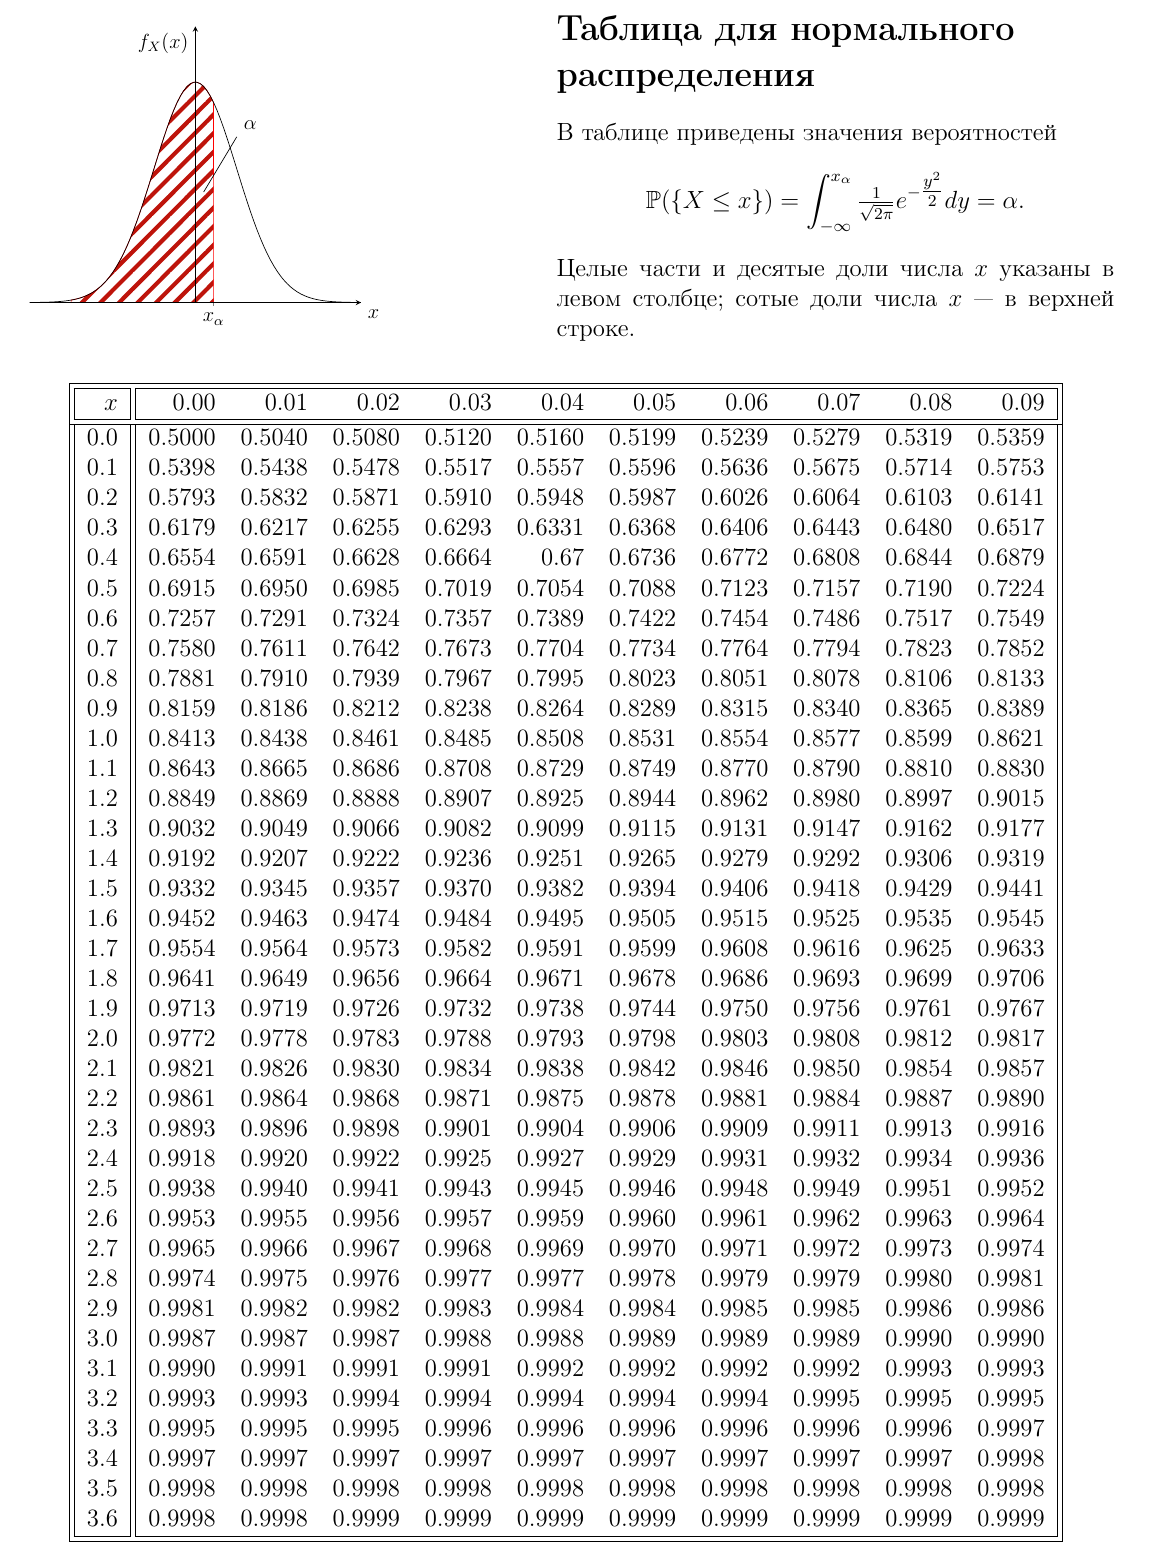
\includegraphics[scale=0.50]{normal_table.png}

\end{enumerate}

\end{document}

% здесь проектируемая часть


